%!TEX TS-program = xelatex
%!TEX encoding = UTF-8 Unicode

\documentclass[8pt]{article}
\usepackage[a4paper]{geometry}
\usepackage[english]{babel}
\usepackage{amssymb,amsthm,amsmath}
%\usepackage{xltxtra}
%\usepackage{stmaryrd}
\usepackage{tikz}
\usepackage{graphicx}
\usepackage{listings}
\usepackage{color}

\graphicspath{ {./images/} }

\definecolor{universityred}{RGB}{147,25,50}
\definecolor{complementaryb}{RGB}{25,147,122}
\definecolor{complementaryo}{RGB}{246,152,84}
\definecolor{complementaryg}{RGB}{110,147,25}

\lstset{
	extendedchars=true,
	showstringspaces=false,
	escapeinside=``,
	keywordstyle=\color{blue},
	commentstyle=\color[rgb]{0.133,0.545,0.133},
	columns=flexible,
	language=python,
	tabsize=2,
	basicstyle=\normalsize\selectfont\ttfamily,
	numbers=left,
	frame=lines,
	breaklines=true
}
\geometry{
	left=15mm,
	right=7mm,
	top=7mm,
	bottom=15mm
}
\usepackage{multicol}
\setlength{\columnsep}{1cm}


\begin{document}
\begin{titlepage}
    \begin{center}
        \vspace*{1cm}

        \Huge
        \textbf{SWERC NoteBook}

        \vspace*{0.5cm}
        \LARGE
        \'Equipe SaintGermainDesPrés

        \normalsize
        \vspace*{1.5cm}
        \textbf{Mathilde BONIN, Eyal COHEN, Hugo DEMARET}

        \vspace*{1cm}
        \textbf{Avril 2022}

        \vspace*{2.5cm}

        \LARGE
        \textbf{Ensemble d'algorithmes et techniques de programmation}
        \vspace*{6.6cm}

        
        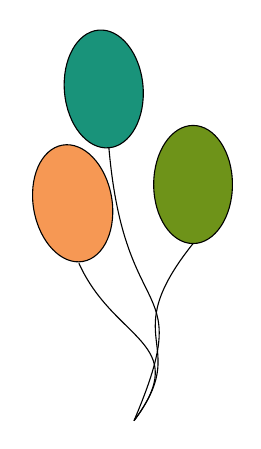
\begin{tikzpicture}
            \filldraw[fill=complementaryg, draw=black](0,2) ellipse (.5cm and .75cm);
            \draw (-0.75,-1) .. controls (0,0) and (-1.,0) .. (0,1.25);
            \draw (-0.75,-1) .. controls (0,0) and (-1.,0) .. (-1.45,1);
            \draw (-0.75,-1) .. controls (0.1,1) and (-1.,0) .. (-1.1,3);
            \draw[rotate around={10:(0,0)},fill=complementaryo, draw=black] (-1.2,2) ellipse (.5cm and .75cm);
            \draw[rotate around={5:(0,0)},fill=complementaryb, draw=black] (-0.85,3.3) ellipse (.5cm and .75cm);
        \end{tikzpicture}

        
\includegraphics[scale=0.05]{../image/cover_image.png}
        \Large

        \textbf{Université Paris Cité}

        UFR de Mathématiques-Informatique

        2021-2022

    \end{center}
\end{titlepage}
    \section{Configuration}
        \subsection{C/C++}
    \section{Chaînes de caractères}
    \section{Séquences}
    \section{Parcours de graphes}
        \subsection{DFS - Depth First Search}
        {\scriptsize\lstinputlisting{../code/graphes/dfs.py}}
        \subsection{BFS - Breadth First Search}
        {\scriptsize\lstinputlisting{../code/graphes/bfs.py}}
        \subsection{Topological Sort}
        \subsection{Composantes connexes}
        \subsection{Composantes bi-connexe}
        \subsection{Composantes fortement connexe}
        \subsection{2-SAT}
        \subsection{Postier Chinois}
        \subsection{Chemin eulérien}
        \subsection{Chemin le plus court}
            \subsubsection{Poids positif ou nul - Dijkstra}
            \subsubsection{Poids arbitraire - Bellman-Ford}
            \subsubsection{Floyd-Warshall}
    \section{Points et polygones}
        \subsection{Points}
            \subsubsection{Points}
            {\scriptsize\lstinputlisting{../code/points/point.py}}
            \subsubsection{Cross-product}
            {\scriptsize\lstinputlisting{../code/points/crossproduct.py}}
            \subsubsection{Direction}
            {\scriptsize\lstinputlisting{../code/points/direction.py}}
        \subsection{Enveloppe convexe}
            Complexité : $\mathcal{O}(n \log(n))$
            {\scriptsize\lstinputlisting{../code/points/jarvismarch.py}}
        \subsection{Aire d'un polygone}
        \textit{Uniquement pour les polygones simples. Réduire à des composantes simples sinon.}
        $A = \frac{1}{2} \sum_{i=0}^{n-1}\left(x_{i}x_{i+1} - x_{i+1}y_{i}\right)$
        {\scriptsize\lstinputlisting{../code/points/polygonearea.py}}
        \subsection{Points entiers dans un polygone}
            \subsubsection{Sur le contour}
            \subsubsection{Dans le polygone}
                Théorème de Pick :
                $P = n_{i} + \frac{n_{b}}{2}-1$
        \subsection{Paire de points les plus proches}
    \section{Ensembles}
        \subsection{Rendu de monnaie}
        Problème NP-Complet.
        {\scriptsize\lstinputlisting{../code/ensembles/coin.py}}
        \subsection{Sac à dos}
        Problème NP-Complet.
        {\scriptsize\lstinputlisting{../code/ensembles/knapsack.py}}
        \subsection{k-somme}
    \section{Calculs}
        \subsection{PGCD}
        {\scriptsize\lstinputlisting{../code/calculs/pgcd.py}}
        \subsection{Coefficients de Bézout}
        {\scriptsize\lstinputlisting{../code/calculs/bezout.py}}
        \subsection{Coefficients binomiaux}
        {\scriptsize\lstinputlisting{../code/calculs/binom.py}}
\end{document}